\documentclass[a4paper]{article}
\usepackage[english]{babel}
\usepackage[utf8x]{inputenc}
\usepackage[T1]{fontenc}
\usepackage{listings}
\usepackage[a4paper,top=2cm,bottom=2cm,left=1.35cm,right=2cm,marginparwidth=1.75cm]{geometry}
\usepackage{amsmath}
\usepackage{graphicx}
\usepackage[colorinlistoftodos]{todonotes}
\usepackage[colorlinks=true, allcolors=blue]{hyperref}
\usepackage{wasysym} % smileys
\setlength\parindent{0pt} % indent

% my commands:
\newcommand{\n}{\newline}
\newcommand{\da}{\hspace{0.15cm}\text{d}\alpha}
\newcommand{\dx}{\hspace{0.15cm}\text{d}x}
\newcommand{\dz}{\hspace{0.15cm}\text{d}z}
\newcommand{\al}{\alpha}
\newcommand{\tab}{\hspace{1cm}}
\begin{document}
\text{}\vspace{-0.1cm}
{\fontfamily{pbk}\fontsize{12}{15}\selectfont \hspace{-0.5cm}\text{6. domácí úkol | Vilém Zouhar}}

\section{}
Elipsa je definovaná buď implicitně: $\frac{x^2}{a^2}+\frac{y^2}{b^2}=1$, nebo parametricky: $x = a\cdot cos(\alpha);\hspace{0.4cm} y = b\cdot sin(\alpha)$. Pro výpočet plochy pod křivkou bude parametrická definice mnohem přívětivější.

\begin{align*}
	& x = \phi(\alpha) = a\cdot \cos(\alpha) \hspace{1cm} y = \psi(\alpha) = b\cdot \sin(\alpha) \\
	& \phi'(\alpha) = -a\cdot \sin(\alpha) \hspace{1.3cm} \psi'(\alpha) = b\cdot \cos(\alpha) \\
	& \\
	& \text{Budeme zkoumat pouze jednu čtvrtinu elipsy, tedy meze $\frac{\pi}{2}$ a $0$. Je však třeba vyřešit smysl úhlu, tedy uspořádání mezí.} \\
	& \hspace{3.5cm}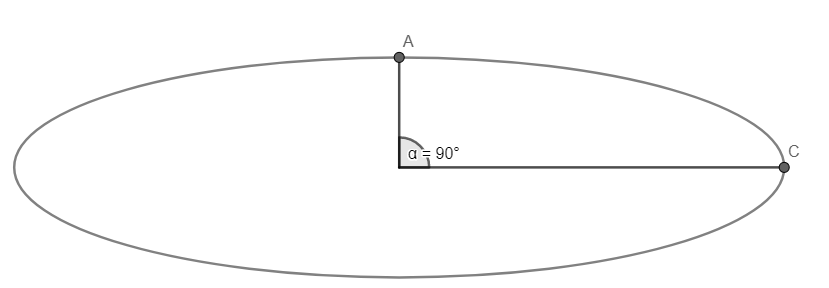
\includegraphics[width=13cm]{ellipse} \\
	& \text{Pro $\alpha = 0$ defijnuje parametrické vyjádření bod $B$, pro $\alpha = \frac{\pi}{2}$ se definuje bod $A$. Abychom šli ve směru osy x,} \\
	& \text{potřebujeme integrovat od $\alpha = \frac{\pi}{2}$ po $\alpha = 0$: } \int_\frac{\pi}{2}^0 b\cdot \sin(\alpha) \cdot a (-1) \sin(\alpha) \da = ab \cdot \int^\frac{\pi}{2}_0 \sin^2(\alpha) \da \\
	& \tab I = \int \sin^2(\al) \da = [\textit{per partes}] = -\sin(\al)\cos(\al) + \int \cos^2(\al) \da = -\sin(\al)\cos(\al) + \int 1 \da - \int \sin^2(\al) \da \\
	& \tab \Rightarrow 2I = -\sin(\al)\cos(\al) + \al + Q \Rightarrow \int \sin^(\al) \da = \frac{-\sin(\al)\cos(\al) + \al}{2} + C \\
	& ab \cdot \int^\frac{\pi}{2}_0 \sin^2(\alpha) \da = ab \cdot \bigg[\frac{-\sin(\al)\cos(\al) + \al}{2}\bigg]_0^\frac{\pi}{2} = ab \bigg[\frac{0+\frac{\pi}{2}}{2}-\frac{0+0}{2}\bigg] = ab\frac{\pi}{4} \\
	& \text{Tím jsme vypočítali jednu čtvrtinu, tedy celkový obsah je: } \pi ab
\end{align*}

\section{}
\begin{align*}
	& y = \frac{a}{2}(e^{x/a} + e^{-x/a}), \hspace{0.15cm} y' = \frac{e^{x/a} - e^{-x/a}}{2}, \hspace{0.15cm} (y')^2 = \frac{e^{2x/a} + e^{-2x/a}-2}{4}, \hspace{0.15cm} 1+(y')^2 = \frac{e^{2x/a} + e^{-2x/a}+2}{4} = \bigg( \frac{e^{x/a} + e^{-x/a}}{2}\bigg)^2 \\
	& \Rightarrow \sqrt{1+(y')^2} = |\frac{e^{x/a} + e^{-x/a}}{2}| = \frac{e^{x/a} + e^{-x/a}}{2} = \cosh(x/a) \\
	& \int \frac{e^{x/a} + e^{-x/a}}{2} \dx = \frac{1}{2} \int e^{x/a} \dx + \frac{1}{2} \int e^{-x/a} \dx =  [\textit{sub. $z=x/a$}] = \frac{a}{2} \int e^{z} \dz + \frac{a}{2} \int e^{-z} \dz = \frac{a}{2} e^{z} - \frac{a}{2} e^{-z} + C =  \\
	& \frac{a}{2} e^{x/a} - \frac{a}{2} e^{-x/a} + C =  a \sinh(x/a) + C \\
	& \text{Délka křivky: } \int_0^\gamma \big[ \frac{e^{x/a} + e^{-x/a}}{2} \big] \dx = \big[ \frac{a}{2} e^{x/a} - \frac{a}{2} e^{-x/a} \big]_0^\gamma = \frac{a}{2}  \big[ e^{x/a} - e^{-x/a} \big]_0^\gamma = \frac{a}{2} [ e^{\gamma/a} - e^{-\gamma/a} ] = a \sinh(\gamma/a)
\end{align*}

\pagebreak
\section{}
Kružnice posunutá ve směru osy $y$ je popsaná implicitně: $(y-R)^2 + x^2 = r^2$ a můžeme ji rozdělit na: \\ $y_{+1}=\sqrt{r^2-x^2} +R, \hspace{0.15cm} y_{-1}=-\sqrt{r^2-x^2} +R$, obecně se znamínkem $s$: $y_s = s\sqrt{r^2-x^2} +R \hspace{0.5cm}(s = \pm1)$ \\
Pro $s = +1$, se jedná o červenou (horní) křivku, pro $s = -1$ o modrou (spodní): \\
\text{}\hspace{5.5cm}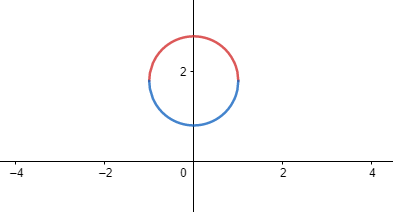
\includegraphics[width=7cm]{circle} \\
Pokud bychom si představili obsah pod červenou křivkou a ten rotovali kolem osy $x$, pak bychom dostali torus bez díry uprostřed (objem $V_{+1}$). To spravíme tak, že od původního objemu odečteme objem vzniklý rotací obsahu pod modrou křivkou kolem osy $x$ (objem $V_{-1}$). Integrály pro výpočet budou velmi podobné a spousta členů se od sebe odečte, proto budeme hned ze začátku dělat rozdíl dvou integrálů. Navíc si upravíme meze vždy jen polovinu (od $0$ po $r$) a celkový objem vynásobíme dvěmi (neboť křivky jsou symetrické podle osy $y$): \\
\begin{align*}
	& V = V_{+1} - V_{-1} = \bigg[ 2\pi \int_0^r (+1\sqrt{r^2-x^2} +R)^2 \dx - 2\pi \int_0^r (-1\sqrt{r^2-x^2} +R)^2 \dx\bigg] \\
	& = [\textit{z linearity integrálů se členy odečtou}] = 2\pi \bigg[ \int_0^r 2R\sqrt{r^2-x^2}  \dx - \int_0^r -2R\sqrt{r^2-x^2} \dx\bigg] \\
	& = 8\pi R \int_0^r \sqrt{r^2-x^2}  \dx = [\textit{substituce $z = x/r$}] = 8\pi Rr^2 \int_0^1 \sqrt{1-z^2} \dz = \\
	& = [\textit{sub. $z=\sin(\al),\hspace{0.15cm} "\hspace{-0.15cm}\dz = \cos(\al) \da"$}] =  8\pi Rr^2 \int_0^\frac{\pi}{2} \sqrt{1-\sin^2(\al)} \cos(\al) \da = \\
	& = 8\pi Rr^2 \bigg[ \int_0^\frac{\pi}{2} 1 \da - \int_0^\frac{\pi}{2} \sin^2(\al) \da \bigg] =  8\pi Rr^2 \bigg[\al - \frac{-\sin(\al)\cos(\al) + \al}{2} \bigg]_0^\frac{\pi}{2} \textit{\hspace{0.15cm}(výpočet $\int \sin^2(x) \dx$ z 1. příkladu)} \\
	& 8\pi Rr^2 \bigg[\frac{\sin(\al)\cos(\al) + \al}{2} \bigg]_0^\frac{\pi}{2} = 8\pi Rr^2 \bigg[\frac{0 + \frac{\pi}{2}}{2}-0 \bigg] = 2\pi^2 Rr^2
\end{align*}
\end{document}
